\documentclass[helvetica]{seminar} 
\input{xy}
\xyoption{all}
\usepackage{graphicx} 
\usepackage{slidesec} 
\usepackage{url}
\usepackage[framemethod=TikZ]{mdframed}
\usepackage{color}
\usepackage[normalem]{ulem}  

\def\dash---{\unskip\kern.16667em---\penalty\exhyphenpenalty\hskip.16667em\ignorespaces}
\long\def\symbolfootnote[#1]#2{\begingroup%
\def\thefootnote{\fnsymbol{footnote}}\footnote[#1]{#2}\endgroup}

% to fix problems making landscape seminar pdfs
% Letter...
\pdfpagewidth=11truein
\pdfpageheight=8.5truein
\pdfhorigin=1truein     % default value(?), but doesn't work without
\pdfvorigin=1truein     % default value(?), but doesn't work without
% A4
%\pdfpagewidth=297truemm % your milage may vary....
%\pdfpageheight=210truemm
%\pdfhorigin=1truein     % default value(?), but doesn't work without
%\pdfvorigin=1truein     % default value(?), but doesn't work without


\renewcommand{\familydefault}{\sfdefault}  
 
\input{seminar.bug} 
\input{seminar.bg2} % See the Seminar bugs list 
 
\slideframe{none} 
 
 
\usepackage{fancyhdr} 
 
% Headers and footers personalization using the `fancyhdr' package 
\fancyhf{} % Clear all fields 
\renewcommand{\headrulewidth}{0mm} 
\renewcommand{\footrulewidth}{0.1mm} 
 
\fancyfoot[L]{\tiny IETF 96} 
\fancyfoot[C]{\tiny TLS}
\fancyfoot[R]{\tiny \theslide} 
 
 
% To center horizontally the headers and footers (see seminar.bug) 
\renewcommand{\headwidth}{\textwidth} 

% To adjust the frame length to the header and footer ones 
\autoslidemarginstrue 
\pagestyle{fancy} 
 

\newcommand{\heading}[1]{% 
  \begin{center} 
    \large\bf 
    #1 
  \end{center} 
  \vspace{.4 in}} 



\begin{document}

\begin{slide}
\begin{center}
\vspace{.5 in}
\LARGE{{\bf}TLS 1.3\\{\small \verb^draft-ietf-tls-tls13-18^}}\\
\vspace{.2in}
\large{
\begin{tabular}{c}
Eric Rescorla\\
Mozilla\\
\url{ekr@rtfm.com}
\end{tabular}
}
\end{center}
\end{slide}

\centerslidesfalse 

\begin{slide}
\heading{Agenda}

\begin{itemize}
\item Status
\item WGLC issues
\item Timeline
\end{itemize}

\end{slide}


\begin{slide}
\heading{Status}

\begin{itemize}
\item In WGLC with: draft-ietf-tls-tls13-18
\item Quite a few interoperable implementations
  \begin{itemize}
  \item draft-16 in Firefox Nightly, Chrome Dev/Canary, Cloudflare live
  \item draft-18 in NSS, BoringSSL (under review), TLS-Tris (Cloudflare), Mint, Fizz (Facebook)
  \item Other implementations under development
  \end{itemize}
\end{itemize}
\end{slide}

\begin{slide}
\heading{Interop Matrix}

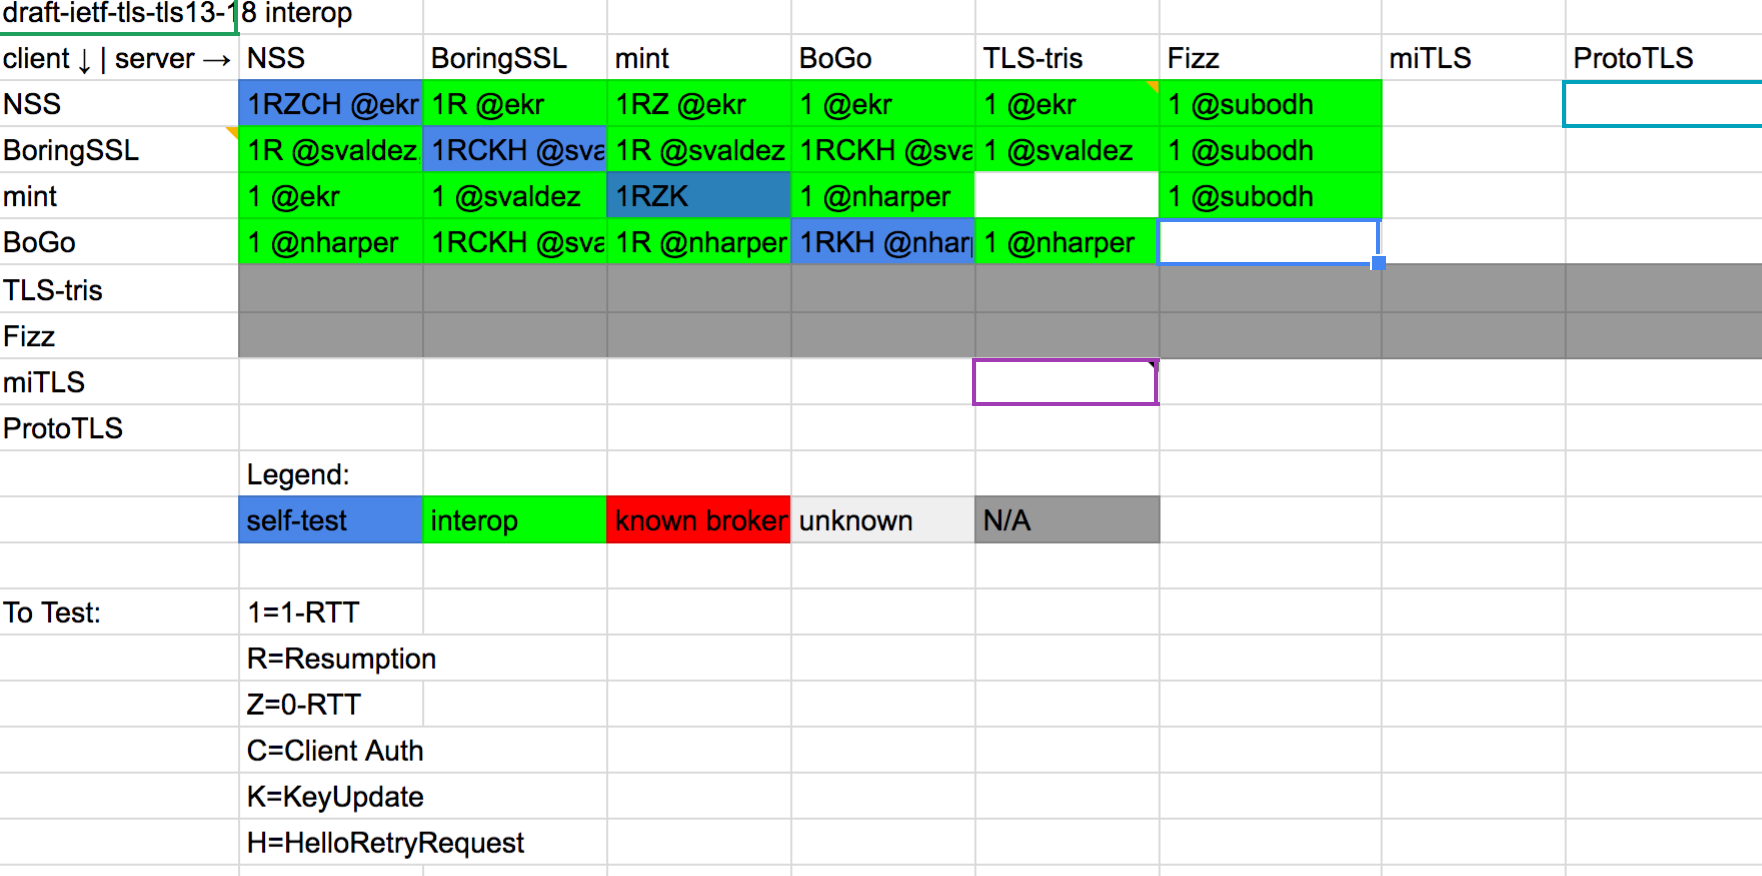
\includegraphics[width=4in]{interop}
\end{slide}


\begin{slide}
\heading{PR\#748: Forbid negotiating $<$ TLS 1.2 with ``supported\_versions''}

\begin{itemize}
\item Draft says that if ``supported\_versions'' is present, it's the sole version negotiation mechanism
  \begin{itemize}
  \item But you should list all the versions you support
  \item In principle possible to negotiate TLS 1.1 via this mechanism
  \end{itemize}
\item Alternate design: require at least TLS 1.2 if you offer TLS 1.3
  \begin{itemize}
  \item Forbid listing any value $<$ TLS 1.2 as client
  \item Forbid negotiating any value $<$ TLS 1.2 on server
  \end{itemize}
\end{itemize}
\end{slide}


\begin{slide}
\heading{Issue\#758: Exporters should call Hash() before HKDF-Expand-Label()}

\vspace{-6ex}
{\scriptsize
\begin{verbatim}
    HKDF-Expand-Label(Secret, Label, HashValue, Length) =
         HKDF-Expand(Secret, HkdfLabel, Length)

    struct {
        uint16 length = Length;
        opaque label<9..255> = "TLS 1.3, " + Label;
        opaque hash_value<0..255> = HashValue;
    } HkdfLabel;
\end{verbatim}
}

\begin{itemize}
\item Exporters are defined as;
\end{itemize}

{\scriptsize
\begin{verbatim}
    HKDF-Expand-Label(Secret, label, context_value, key_length)
\end{verbatim}
}

\begin{itemize}
\item This means you pass ``context\_value'' as ``hash''
\item Confusing and imposes a 255-byte limit.
\item Proposal:
\end{itemize}

{\scriptsize
\begin{verbatim}
    HKDF-Expand-Label(Secret, label, Hash(context_value), key_length)
\end{verbatim}
}
\end{slide}


\begin{slide}
\heading{Issue\#760: Certificate extension rules and client certs}

\begin{itemize}
\item In draft-18 we put extensions in Certificate
  \begin{itemize}
  \item Gated on ClientHello extensions
  \item This doesn't make any sense for the cert for client authentication
  \end{itemize}

\item We have extensions in CertificateRequest
  \begin{itemize}
  \item But they just filter on OID/value pair
  \item Proposed resolution: add real extensions to CertificateRequest
  \end{itemize}
\end{itemize}
\end{slide}

\begin{slide}
\heading{Issue\#760: CertificateRequest}

\vspace{-5ex}
{\scriptsize
\begin{verbatim}
 struct {
       opaque certificate_request_context<0..2^8-1>;
       SignatureScheme
         supported_signature_algorithms<2..2^16-2>;
       DistinguishedName certificate_authorities<0..2^16-1>;
       Extension certificate_extensions<0..2^16-1>;
   } CertificateRequest;

   struct {
       opaque certificate_extension_oid<1..2^8-1>;
       opaque certificate_extension_values<0..2^16-1>;
   } OIDFilter;

   struct {
     OIDFilter filters<0..2^16-1>;
   } OIDFilterExtension;
\end{verbatim}
}

\begin{itemize}
\item Previous CertificateRequest.extensions now are OID extensions
\end{itemize}
\end{slide}

\begin{slide}
\heading{Issue\#760: CertificateRequest extension variations}

\begin{itemize}
\item Replace OIDs with extension IDs and flattten list
\item Have two lists (OIDs and usual extensions)
\item[]
\item We should also make certificate\_authorities an extension
\end{itemize}
\end{slide}


\begin{slide}
\heading{Record Header}

{\scriptsize
\begin{verbatim}
       struct {
           ContentType opaque_type = 23; /* application_data */
           ProtocolVersion legacy_record_version = 0x0301; /* TLS v1.x */
           ...
       } TLSCiphertext;
\end{verbatim}

\begin{itemize}
\item This is three bytes of waste.
  \begin{itemize}
  \item Would like to get rid of it
  \item Questions about interop (with passive inspection middleboxes)
  \end{itemize}
\item Subtle point about 0-RTT failure transition
  \begin{itemize}
  \item Steal a bit from the header
  \end{itemize}
\item Proposal in PR\#762
  \begin{itemize}
  \item We will take compat measurements in the next month or two
  \item WG can then decide
  \end{itemize}
\end{itemize}
}
\end{slide}

\begin{slide}
\heading{Longer key lifetimes}

\vspace{-2ex}
{\scriptsize
\begin{verbatim}
Regardless of the actual record size, each 128-bit block encryption is
performed with a unique 128-bit counter which is formed by the 96-bit
IV and the 32-bit counter_block value called CB in NIST SP 800-38D
under a given key as long as the number of encrypted records is not
more than 2^64.

Assuming a user would like to limit the probability of a collision
among 128-bit ciphertext-blocks under 1/2^32, the data limit of the
ciphertext ( or plaintext) is 2^(96/2) (= 2^48) 128-bit blocks which
is 2^64 bytes.

Reading the 2nd paragraph of section 5.5, a user might feel that
he/she needs to rekey a lot more quicker than he/she needs. Putting an
unnecessarily low data limit of 2^24.5 full-size records (2^38.5
bytes) also creates an incorrect negative impression (in my opinion)
about GCM.

I would like to request the working group to consider to revise the
text.
\end{verbatim}

\begin{itemize}
\item Anyone persuaded?
\end{itemize}
}

\end{slide}


\begin{slide}
\heading{PR\#763: EC Point Validation}

\begin{itemize}
\item Requires point validation for remote key shares
\item Specifies the procedure for NIST curves
\end{itemize}

\end{slide}


\begin{slide}
\heading{Timeline}

\begin{tabular}{l l}
Nov 20 & WGLC Ends \\
Dec 1 & draft-19 with all WGLC comments \\
Dec 31 & Results of record header experiment \\
Jan 15 & draft-20 \\
Jan 31 & End of cryptographic review period \\
Feb 10 & Draft-20 (if needed) and pub request \\
\end{tabular}

\end{slide}


\end{document} 
